%-----------------------------------------------
% Dateiname: InstallTYPO3.tex
% Autor    : Stefano Kowalke <blueduck@gmx.net>
% Lizenz   : BSD
%-----------------------------------------------
\section{Vorbereitung}
\label{prototype:sec:preparation}

\subsection{Installation von TYPO3 CMS}
\label{prototype:subsec:installTYPO3}
TYPO3 CMS wurde auf dem lokalen Rechner per \textit{GIT} in der Entwicklerversion 6.2.x-dev unter \url{thesis.dev} installiert. TYPO3 CMS 6.2 stellte die zum Zeitpunkt der Implementierung aktuelle Version dar. Die Entwicklerversion wurde gewählt, um von der fortlaufenden Weiterentwicklung des Systems zu profitieren. \textit{GIT} wurde verwendet, damit der Code einfacher aktualisierbar war und eigene Änderungen daran nachvollzogen und dokumentiert werden konnten.

Abbildung~\ref{lst:thesisDevFolders} zeigt die Verzeichnisstruktur nachdem das System installiert und alle notwendigen Verzeichnisse und Symlinks erstellt wurden:

\begin{figure}[H]
\begin{Verbatim}[samepage=true]
$ tree -L 2 --dirsfirst
.
├── http
│   ├── fileadmin
│   ├── typo3 -> typo3_src/typo3
│   ├── typo3_src -> ../typo3cms
│   ├── typo3conf
│   ├── uploads
│   └── index.php -> typo3_src/index.php
└── typo3cms
    ├── typo3
    ├── ChangeLog
    ├── GPL.txt
    ├── INSTALL.md
    ├── LICENSE.txt
    ├── NEWS.md
    ├── README.md
    ├── _.htaccess
    ├── composer.json
    └── index.php
\end{Verbatim}
\caption{Die Grundstruktur von \url{thesis.dev}}
\label{lst:thesisDevFolders}
\end{figure}

Das Verzeichnis \pdf{http} wurde per Eintrag in der Apache2 Konfiguration als VirtualHost definiert.

\begin{shcode}
<VirtualHost *:80>¬
DocumentRoot "~/Sites/thesis.dev/http"¬
ServerName thesis.dev¬
</VirtualHost>
\end{shcode}

TYPO3 CMS wurde nach \pdf{typo3cms} installiert, damit dessen Dateien nicht über den Apache ereichbar sind.

Um die Installation unter der Adresse \url{thesis.dev} erreichen zu können, wurde in der Hostdatei ein A-Record angelegt.

\begin{shcode}
sudo sh -c "echo '127.0.0.1 thesis.dev' >> /etc/hosts"
\end{shcode}

Im Anschluß daran wurde eine leere Datenbank mit dem Namen \texttt{thesis} erstellt:

\begin{shcode}
mysql -u root -p
MariaDB [(none)]> create database if not exists thesis;
Query OK, 1 row affected (0.01 sec)
MariaDB [(none)]> quit;
\end{shcode}

Durch das Aufrufen von \url{http://thesis.dev/} im Browser wird der Installationsprozess gestartet, der in fünf Schritten das System installiert.

\subsection{Schritt 1 - Systemcheck}
\label{prototype:subsec:OneSystemcheck}
	Im ersten Schritt (Abb.:~\ref{fig:installTYPO3LegacyStepOne}) prüft das \textit{Install Tool} ob alle Verzeichnisse und Symlinks angelegt wurden und die entsprechenden Benutzerrechte besitzen. Intern werden hier Verzeichnisse wie \pdf{typo3temp} und Dateien wie \pdf{LocalConfiguration.php} angelegt.

\subsection{Schritt 2 - Eingabe der Datenbankdaten}
\label{prototype:subsec:TwoInsertDatabaseData}
	Im zweiten Schritt (Abb.:~\ref{fig:installTYPO3LegacyStepTwo}) werden die Benutzerdaten für die Datenbank eingegeben. Es kann zwischen einer Port- oder Socket-basierten Verbindung ausgewählt werden.

	Wenn anstelle von MySQL ein alternatives \gls{dbms} genutzt werden soll, kann über die Schaltfläche am Ende des Formulars die Systemextension DBAL installiert werden.

\subsection{Schritt 3 - Auswahl der Datenbank}
\label{prototype:subsec:ThreeSelectDatabase}
	Nachdem die Verbindungsdaten eingegeben wurden, versucht TYPO3 CMS eine Verbinung zum \gls{dbms} zu etablieren. Gelingt dies, werden alle verfügbaren Datenbanken abgefragt und aufgelistet (Abb.:~\ref{fig:installTYPO3LegacyStepThree}). Über die Auswahl kann eine leere Datenbank festgelegt werden. Alternativ kann über das Inputfeld eine zu erstellende Datenbank angegeben werden. Mit dem Absenden des Formulars werden die Basistabellen in der Datenbank angelegt.

\subsection{Schritt 4 - Einrichten eines TYPO3 Administrators}
\label{prototype:subsec:FourCreateAdmin}
	In 4. Schritt (Abb.:~\ref{fig:installTYPO3LegacyStepFour}) der Installation wird ein Administrator eingerichtet und es kann ein Name für die Seite vergeben werden.

\subsection{Schritt 5 - Abschluß der Installation}
\label{prototype:subsec:FiveDone}
	Danach ist die Installation abgeschlossen und über die Schaltfläche kann das Backend aufgerufen werden (Abb.:~\ref{fig:installTYPO3LegacyStepFive})

	\begin{figure}[H]
		\begin{subfigure}[b]{0.5\textwidth}
			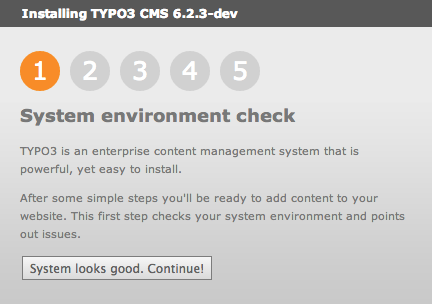
\includegraphics[width=\textwidth]{InstallingTYPO3/DoctrineDBAL/01-SystemEnvironmentCheck.png}
			\caption{Installation TYPO3 CMS - 1. Schritt}
			\label{fig:installTYPO3LegacyStepOne}
		\end{subfigure}%
		~ %add desired spacing between images, e. g. ~, \quad, \qquad, \hfill etc.
	%(or a blank line to force the subfigure onto a new line)
		\begin{subfigure}[b]{0.5\textwidth}
			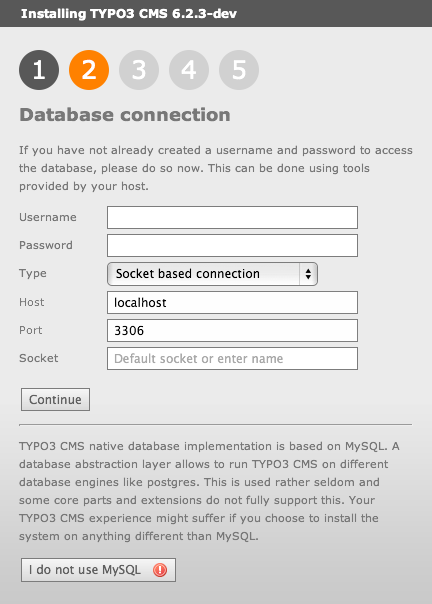
\includegraphics[width=\textwidth]{InstallingTYPO3/Legacy/02-DatabaseConnectionLegacy.png}
			\caption{Installation TYPO3 CMS - 2. Schritt}
			\label{fig:installTYPO3LegacyStepTwo}
		\end{subfigure}
		~ %add desired spacing between images, e. g. ~, \quad, \qquad, \hfill etc.
	%(or a blank line to force the subfigure onto a new line)
		\begin{subfigure}[b]{0.5\textwidth}
			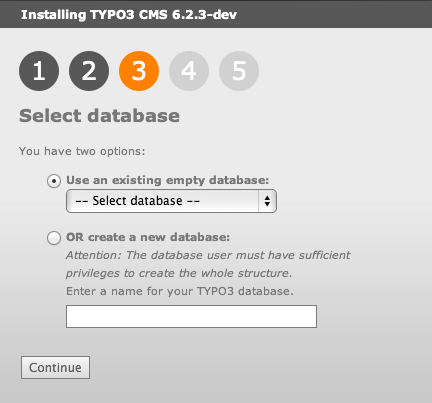
\includegraphics[width=\textwidth]{InstallingTYPO3/Legacy/03-SelectDatabaseLegacy.png}
			\caption{Installation TYPO3 CMS - 3. Schritt}
			\label{fig:installTYPO3LegacyStepThree}
		\end{subfigure}%
		~ %add desired spacing between images, e. g. ~, \quad, \qquad, \hfill etc.
	%(or a blank line to force the subfigure onto a new line)
		\begin{subfigure}[b]{0.5\textwidth}
			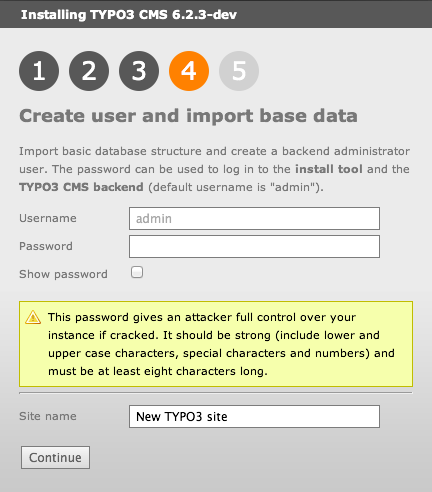
\includegraphics[width=\textwidth]{InstallingTYPO3/Legacy/04-CreateUserAndImportBaseDataLegacy.png}
			\caption{Installation TYPO3 CMS - 4. Schritt}
			\label{fig:installTYPO3LegacyStepFour}
		\end{subfigure}
		~ %add desired spacing between images, e. g. ~, \quad, \qquad, \hfill etc.
	%(or a blank line to force the subfigure onto a new line)
		\begin{subfigure}[b]{0.5\textwidth}
			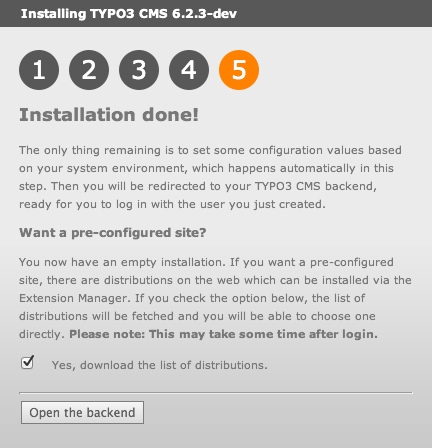
\includegraphics[width=\textwidth]{InstallingTYPO3/Legacy/05-InstallationDoneLegacy.png}
			\caption{Installation TYPO3 CMS - 5. Schritt}
			\label{fig:installTYPO3LegacyStepFive}
		\end{subfigure}%
		\caption{Installation von TYPO3 CMS}
		\label{fig:installationOfTYPO3}
	\end{figure}

\subsection{Implementation von Unit Tests der alten Datenbank API}
\label{prototype:sec:createTestForOldAPI}
Um zu gewährleisten, dass TYPO3 CMS sowohl mit der alten API - die von dem Prototypen zur Verfügung gesellt wird - als auch mit der neuen API kompatibel ist, müssen Untit Tests für die alte Datenbank API geschrieben werden.

Zur Ausführung der Unit Tests wird die Extension \textit{PHPUnit} benötigt, welche das gleichnamige Testing Framework \textit{PHPUnit\footnote{\url{http://www.phpunit.de}}} zur Verfügung und einen einen graphischen Testrunner im Backend mitbringt. Sie wird über den Extension Manager installiert.

Die alte Datenbank API verfügt zur dem Zeitpunkt der Erstelltung des Prototypen über 40 Tests mit 49 Assertions, welche jedoch lediglich Hilfsmethoden testen. Im Laufe der Arbeit wurden wurden 68 Tests implementiert, die alle Methoden testen. Die Abbildung~\ref{fig:executeUnitTestsForOldAPI} zeigt die Ausführung der von TYPO3 CMS mitgelieferten Unit Tests; Abbildung~\ref{fig:executeNewUnitTestsForOldAPI} zeigt die Ausführung der neu implementierten sowie der alten Tests.

\begin{figure}[H]
    \centering
    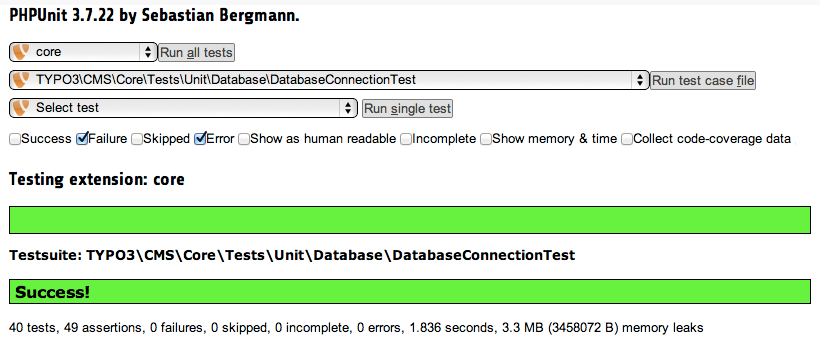
\includegraphics[scale=0.5]{TYPO3/DatabaseConnectionUnitTestsLegacy.png}
    \caption{Ausführung der vorhandenen Unit Tests für die alte Datenbank API}
    \label{fig:executeUnitTestsForOldAPI}
\end{figure}

\begin{figure}[H]
    \centering
    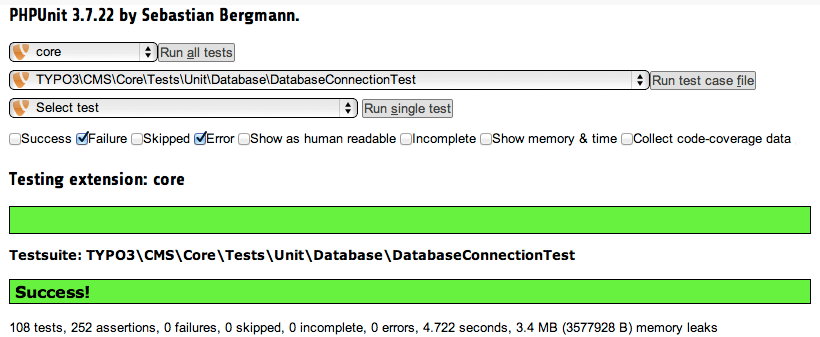
\includegraphics[scale=0.5]{TYPO3/DatabaseConnectionAddedUnitTestsLegacy.png}
    \caption{Ausführung der vorhandenen und hinzugefügten Unit Tests für die alte Datenbank API}
    \label{fig:executeNewUnitTestsForOldAPI}
\end{figure}
